
\section{Resilience in the Homogeneous Model} \label{sec:architectures}

The emergence of power laws for cascading failures in supply chain graphs, as we show in \cref{theorem:power_laws}, indicates the need to define a resilience metric. It is important to have a suitable resilience metric to understand the behavior of complex systems and identify potential vulnerabilities. There are many different ways to define and measure resilience, and which metric is most appropriate will depend on the specific system being studied and the goals of the analysis. Some common approaches to defining resilience include looking at the system's ability to recover from disturbances, absorb or adapt to change, and maintain function in the face of stress or disruption.

In our percolation model, ideally, a ``more resilient'' network is a network that can withstand larger shocks, which are associated with larger percolation probabilities $x$. Therefore, it is natural to assume that in a resilient network, we want to find the maximum value that the percolation probability $x$ can get in order for a ``large'' fraction of the items to survive almost surely. Formally, for $\varepsilon \in (0, 1)$, the \emph{resilience} of a product graph (possibly random) $\cG$ is defined as follows.

\begin{tcolorbox}
\vspace{-20pt}
\begin{align} \label{eq:resilience_iid}
    R_{\cG} (\varepsilon) = \sup \left \{ x \in (0, 1) : \Pr_{\cG,x} { \left [S \ge (1 - \varepsilon)  {K} \right ]} \ge 1 - \frac {1} {K} \right \},
\end{align} 
\end{tcolorbox}

$R_{\cG} (\varepsilon)$ corresponds to the maximum percolation probability for which, at most $\varepsilon K$ products fail with a probability at least $1-1/K$ that increases to one as $K \to \infty$. The expectation $\ev {\cG} {\cdot}$ corresponds to the randomness of the graph generation process and the probability $\Pr_{\cG, x} [\cdot]$ corresponds to the joint randomness of the percolation and the edges of the graph. In the case of $\mathsf{rdag}(K, p)$, our lower bound on $x$ in Appendix \ref{app:analytical_lower_bound} to ensure $\Pr [F \ge \varepsilon K] = O(1/K)$ is also a lower bound on the resilience for this particular architecture. 

We make a distinction between the following two classes of networks: 

\begin{mdefinition}\label{def:resilience-taxonomy}
    A family of production networks $\cG$ indexed by their number of products $K$, is \textbf{resilient} iff $\lim_{K \to \infty} R_{\cG}(\varepsilon) > 0$ for any fixed $\varepsilon \in (0, 1)$, and it is \textbf{fragile} iff $\lim_{K \to \infty} R_{\cG}(\varepsilon) = 0$ for any fixed $\varepsilon \in (0, 1)$.
\end{mdefinition}

That is, the former type of architecture can be characterized as \emph{fragile architecture} since even the smallest failure can devastate the network. The latter can be characterized as \emph{resilient architecture} since it can withstand non-trivial shocks in the limit of $K \to \infty$.

Similarly to existing approaches in random graph theory (cf. \cite{bollobas2001random}), we consider the case where the number of products is large as a means to represent an arbitrarily complex economy. However, we want to note that our results are non-asymptotic, which makes them suitable for real-world supply chains. 

In the sequel, we study a variety of network architectures and derive lower bounds for the resilience of such supply chain architectures. \cref{tab:resiliences} summarizes our results. Briefly, to prove that a supply chain $\cG$ is resilient, it suffices to choose some lower bound percolation probability $\underline R_{\cG}(\varepsilon) \in (0, 1)$ such that $\Pr_{x = \underline R_{\cG}(\varepsilon)} [F \ge \varepsilon K] = O \left ( {1}/{K} \right )$ and prove that, which implies that $\lim_{K \to \infty} R_{\cG}(\varepsilon) > 0$ since $R_{\cG}(\varepsilon) \ge \underline R_{\cG}(\varepsilon)$. Moreover, to prove that architecture is fragile, we prove an upper bound $\overline R_{\cG}(\varepsilon) \in (0, 1)$ on the resilience that goes to 0 as $K \to \infty$. To derive upper bounds, we can use the following lemma, whose proof is deferred to Appendix \ref{app:proof:upper_bound_resilience}. The constant $1/2$ in the following lemma is arbitrary and the proof works for any constant $\theta \in (0, 1)$.

\begin{lemma} \label{lemma:upper_bound_resilience}
    Let $\varepsilon \in (0, 1)$ and let $\overline R_{\cG}(\varepsilon) \in (0, 1)$ be a percolation probability such that $\Pr_{x = \overline R_{\cG}(\varepsilon)} [S \ge (1 - \varepsilon) K] \le \frac 1 2$. Then, for $K \ge 3$, we have $ R_{\cG}(\varepsilon)<\overline R_{\cG}(\varepsilon)$. 
\end{lemma}

As a warm-up, the analysis of \cref{sec:motivation} shows that $\mathsf{rdag}(K, p)$ is a fragile architecture, and therefore we get our first theorem.

\begin{theorem} \label{theorem:rdag_resilience}
    Let $\cG \sim \mathsf{rdag}(K, p)$. Then, as $K \to \infty$, we have $R_{\cG} (\varepsilon) \to 0$.
\end{theorem}

In the next sections, we study various architectures and derive upper and lower bounds of $R_{\cG}(\varepsilon)$. 

\subsection{Parallel Products with Dependencies} \label{sec:parallel_products}


\begin{figure}[t]
    \centering
    \subfigure[$\mathsf{rdag}(K = 3, p)$\label{fig:random_dag_2}]{
    \begin{tikzpicture}[transform shape]
        \Vertex[x=-2, y=0, label=$1$, color=pink]{u1}
        \Vertex[x=0, y=0, label=$2$]{u2}
        \Vertex[x=2, y=0, label=$3$, color=pink]{u3}
        \Edge[Direct, color=black, label=$1- p$, style={dashed}](u1)(u2)
        \Edge[Direct, color=black, label=$p$, ](u2)(u3)
        \Edge[Direct, color=black, label=$p$, bend=30](u1)(u3) 
    \end{tikzpicture}} \quad
    \subfigure[Parallel Products ($\mu = 2$, $m = 3$).\label{fig:parallel_products}]{
    \begin{tikzpicture}[]
        \Vertex[x=-1,y=0,Pseudo]{rz}
        \Vertex[x=4,y=0,Pseudo]{rzz}

        \Vertex[x=-0.25,y=0,Pseudo,label={$\cR$}]{r0}
        \Vertex[x=4.25,y=0,Pseudo]{x}

        \Vertex[x=1,y=0,color=pink]{r1}
        \Vertex[x=2,y=0]{r2}
        \Vertex[x=3,y=0]{r3}

        \Vertex[x=-0.25,y=1.25,Pseudo,label={$\cC$}]{c0}

        \Vertex[x=1.5,y=1.25,color=pink]{c1}
        \Vertex[x=2.5,y=1.25,color=pink]{c2}

        \Edge[color=black,Direct](r1)(c1)
        \Edge[color=black,Direct](r2)(c1)
        \Edge[color=black,Direct](r3)(c1)
        \Edge[color=black,Direct](r1)(c2)
        \Edge[color=black,Direct](r2)(c2)
        \Edge[color=black,Direct](r3)(c2)

        
    \end{tikzpicture}}
    
    %\shrink
    \caption{Production networks of \cref{sec:motivation} and \cref{sec:parallel_products}. Failures are drawn in pink color.}
    \shrink
    \label{fig:parallel_products_rdag}
\end{figure}


The first architecture we study is parallel products (cf. \cite{bimpikis2019supply,willems2008data} for related works that motivate this architecture). Here, our objective is to produce a set $\cC$ of final goods and each requires $m$ inputs (raw materials; source dependencies).  We also introduce supply dependencies among raw materials, assuming that each raw material can supply $\mu$ products. \cref{fig:parallel_products} shows an example of this supply chain together with an instance of the percolation process (the affected nodes are drawn in pink). Here, it is interesting to study both the resilience of the whole graph, i.e., the graph with vertex set $\cC \cup \cR$, as well as the resilience of the final goods $\cC$ alone. We show that if the source dependency $m$ and the supply dependency $\mu$ between the products are independent of $K$, then the production network is resilient. The resilience metric is lower bounded by $\left ( \frac {\varepsilon} {2(\mu+1)m} \right )^{1/n}$ in both cases (final goods alone or together with raw materials), as the number of products goes to infinity. Moreover, if the number of inputs $m$ goes to infinity, the resilience goes to $0$ at rate $O \left ( e^{- \frac {1} {mn}} \right )$, 
% and \textcolor{red}{the resilience of the final goods goes to $0$ at rate $O \left ( e^{- {C^{\frac 1 m}}/{n}} \right )$} for some constant $C \in (0, 1)$. 
Formally, we prove the following for the resilience of the parallel products (proved in Appendix \ref{theorem:parallel_products}): 

\begin{theorem} \label{theorem:parallel_products}
    Let $\cG$ consist of parallel products with $c$ final goods and assume that $r$ raw materials can produce these products, and each raw material supplies at most $\mu$ final goods, and each final good requires at most $m$ raw products. Then, the resilience of the final goods $\cC$ (which corresponds to the highest probability that at least $(1 - \varepsilon) c$ final products survive) satisfies: $\left ( \frac {\varepsilon} {\mu m} + \sqrt {\frac {\log K} {2mK}} \right )^{1/n} \le R_{\cC}(\varepsilon) \le \left ( 1 - \left ( \frac {1 - \varepsilon} 2 \right )^{1/m} \right )^{1/n}$. In addition, the resilience of all products (final and raw) satisfies $\left ( \frac {\varepsilon} {2 (\mu + 1)m} + \sqrt {\frac {\log (K/2)} {2mK}} \right )^{1/n} \le R_{\cG}(\varepsilon) \le \left ( 1 - \frac {1 - \varepsilon} {2 (m + 1)} \right )^{1/n}$. Subsequently, if $\varepsilon, \mu$ and $m$ are independent of $K$, then the resilience is $\Omega \left ( \left ( \frac {\varepsilon} {\mu m} \right )^{1/n} \right )$ and the network is resilient. 
\end{theorem}

% \begin{proofsketch}
%     For brevity, we give an analysis in expectation for $R_{\cC}(\varepsilon)$.  Let $K_\cC = |\cC|$. The high-probability analysis has been deferred to Appendix \ref{app:proof:theorem:parallel_products}, where the lower bound is improved by an additive factor of $\sqrt{\frac {\log K} {2mK}}$ via Chernoff bounds. The analysis for $\cG$ is similar. To show the lower bound, we show that to have at least $\varepsilon K_\cC$ final goods fail in total, we need at least $\varepsilon K_\cC/\mu$ raw materials to fail. The expected number of raw materials that fail is $r x^n \le m K_\cC x^n$, and therefore by equating $\frac {\varepsilon K_{\cC}} \mu$ with $mK_{\cC} x^n$, we get the desired answer. To derive the upper bounds, we simply upper bound the expected number of surviving final goods $\ev {} {S_{\cC}} \le K(1 - x^n)^m$ and apply Markov's inequality and \cref{lemma:upper_bound_resilience}.
% \end{proofsketch}

\subsection{Hierarchical Production Networks}

A supply chain can be organized hierarchically, with different levels representing different stages of the production process. The raw materials or components that go into the production of a product are at the bottom of the hierarchy, and the finished product is at the top. Each level of the hierarchy represents a stage of production in which materials or components are transformed into a more advanced or finished product \citep{elliott2022supply}. This hierarchical structure helps visualize the flow of materials and information throughout the supply chain and identify potential bottlenecks or inefficiencies. Moreover, another possible hierarchy is to produce final goods from a source of raw products. In this section, we study these two hierarchies, which we call \emph{backward} and \emph{forward} (referring to the directions of percolation with respect to network growth), production networks visualized in \cref{fig:tree_percolation}. More specifically, we consider:
\begin{compactitem}
    \item The \emph{backward production network} (\cref{subfig:forward_backward}) at which the tree grows from the root, and then the percolation starts from the leaves and proceeds to the root. For the scope of this paper, we study backward percolation in deterministic $m$-ary trees. In \cref{sec:forward_backward_tree} we prove that, as expected, such supply chains are, in fact, fragile and give lower bounds on resilience. 
    \item The \emph{forward production network} (\cref{subfig:forward_forward}) at which the tree grows from the root, and then the percolation starts from the root and proceeds to the leaves. Here, the production network is generated by a stochastic \emph{branching process}; the Galton-Watson (GW) process. In \cref{sec:forward_forward_tree}, we prove that, under specific conditions, such supply chains are fragile with a non-negative probability and are otherwise resilient.  
\end{compactitem}

\begin{figure}[t]
    \centering
    \subfigure[\label{subfig:forward_backward}]{
    \begin{tikzpicture}[transform shape, scale=0.85]
        \Vertex[x=0, y=0, color=pink]{u1}
        \Vertex[x=1, y=0.5, color=pink]{u3}
        \Vertex[x=1, y=-0.5]{u2}
        \Vertex[x=2, y=-1.5]{u4}
        \Vertex[x=2, y=-0.5]{u5}
        \Vertex[x=2, y=0.5, color=pink]{u6}
        \Vertex[x=2, y=1.5, color=pink]{u7}

        \Edge[color=black, Direct](u2)(u1)
        \Edge[color=black, Direct](u3)(u1)
        \Edge[color=black, Direct](u4)(u2)
        \Edge[color=black, Direct](u5)(u2)
        \Edge[color=black, Direct](u6)(u3)
        \Edge[color=black, Direct](u7)(u3)

        \Vertex[x=-2, y=-2, Pseudo]{x1}
        \Vertex[x=3.5, y=-2, Pseudo]{x2}
        \Vertex[x=-2, y=2, Pseudo]{y1}
        \Vertex[x=3.5, y=2, Pseudo]{y2}

        \Edge[color=blue, Direct, label={Tree Growth}](x1)(x2)
        \Edge[color=red, Direct, label={Percolation}](y2)(y1)

        
    \end{tikzpicture}} 
    \subfigure[\label{subfig:forward_forward}]{
    \begin{tikzpicture}[transform shape, scale=0.85]

        \Vertex[x=0, y=0]{u1}
        \Vertex[x=1, y=0.5]{u3}
        \Vertex[x=1, y=-0.5, color=pink]{u2}
        \Vertex[x=2, y=-1.5, color=pink]{u4}
        \Vertex[x=2, y=-0.5, color=pink]{u5}
        % \Vertex[x=2, y=0.5, color=pink]{u6}
        % \Vertex[x=2, y=1.5, color=pink]{u7}

        \Edge[color=black, Direct](u1)(u2)
        \Edge[color=black, Direct](u1)(u3)
        \Edge[color=black, Direct](u2)(u4)
        \Edge[color=black, Direct](u2)(u5)
        % \Edge[color=black, Direct](u3)(u6)
        % \Edge[color=black, Direct](u3)(u7)

        \Vertex[x=-2, y=-2, Pseudo]{x1}
        \Vertex[x=3.5, y=-2, Pseudo]{x2}
        \Vertex[x=-2, y=2, Pseudo]{y1}
        \Vertex[x=3.5, y=2, Pseudo]{y2}

        \Edge[color=blue, Direct, label={Tree Growth}](x1)(x2)
        \Edge[color=red, Direct, label={Percolation}](y1)(y2)
    \end{tikzpicture}}
    \subfigure[\label{fig:gw_subcritical}]{\includegraphics[width=0.5\textwidth]{figures/gw_resilience_subcritical.pdf}}
    %\shrink
    
    \caption{(a, b): Backward and Forward Networks. Node failures are drawn in pink. (c): Resilience bounds for a subcritical GW process with branching distribution as a function of $\mu$; note the decreasing trends in both upper and lower bounds, $\ev {\cG} {\overline R_{\cG}(\varepsilon)}$ and $\ev {\cG} {\underline R_{\cG}(\varepsilon)}$, with increasing $\mu$.}
    \label{fig:tree_percolation}
    \shrink
\end{figure}

\subsubsection{Backward Production Network} \label{sec:forward_backward_tree}

In the case of the backward production network, we consider an $m$-ary tree with height $D$ and fanout $m \ge 1$. The levels of the tree correspond to the ``tiers'' with raw materials placed in the tier $D$ and more complicated products placed in higher tiers. Each product has $n$ potential suppliers, and each product in the tier $d \in [D - 1]$ has exactly $|\cN(i)| = m$ inputs from the tier $d + 1$. Tier $d = D$, which corresponds to the raw products, has no inputs. \cref{subfig:forward_backward} shows how the percolation process evolves in a tree with $m = 2$ and $D = 3$, where failures (drawn in pink) propagate from the two faulty raw materials to the root.  

In addition to the power law result (\cref{theorem:power_laws}), the case of the $m$-ary tree is another example that motivates the resiliency measure $R_{\cG}(\varepsilon)$. Specifically, let us think about the probability of a catastrophic failure in a tree, that is, one that affects a substantial proportion of the suppliers in the production network. A raw material failing to be produced can cause its parent product not to be produced and inductively create a cascade up to the root. The complete cascade will start from the failed product in tier $D - 1$ since some products in tier $D - 1$ may be made if their corresponding raw materials are produced. However, no product can be produced from tier $D - 2$ onward. As a result, only $o(K)$ products survive. The probability of such an event equals: 
\begin{align} \label{eq:quick}
    \Pr [S = o(K)]  \ge \Pr [\text{$\ge 1$ raw material malfunctions}] = 1 - (1 - x^n)^{m^{D - 1}} \ge 1 - e^{-x^n m^{D - 1}}. 
\end{align}
It is easy to see that if $x = \Omega \left ( \left ( {m \log K}/{K} \right )^{1/n} \right )$, then a catastrophe occurs with a high probability in the tree structure, meaning that failure probabilities as small as $\left (  {m \log K}/ {K} \right )^{1/n} + o(1)$ can cause catastrophes with probability approaching one (and therefore the backward hierarchical production network is a fragile architecture). Therefore, it is interesting to study cases where such a scenario does not happen; on the contrary, we have many products that survive. The following theorem formalizes the lower bounds and provides an additional upper bound for the resilience of the backward production network (proved in Appendix \ref{app:proof:theorem:tree_resilience}). 

\begin{theorem} \label{theorem:tree_resilience}
    Let $\cG$ be a backward production network with fanout $m$ and depth $D$. Then, 
    \begin{align}
        \left [ 1 - \left ( 1 - \frac 1 {K} \right )^{\frac {1} {(1 - \varepsilon) K}} \right ]^{1/n} \le R_{\cG}(\varepsilon) \le \begin{cases}
            \left ( \frac {2} {K (1 - \varepsilon)}\right )^{1/n} = \left ( \frac {2} {D (1 - \varepsilon)}\right )^{1/n}, & m = 1 \\
            \left ( \frac {(1 - \varepsilon) \log m} {\log K} \right )^{1/n} \asymp \left ( \frac {(1 - \varepsilon)} {D} \right )^{1/n}, & m \ge 2
        \end{cases}.
    \end{align}
    Therefore, the network is fragile. 
\end{theorem}

% \begin{proofsketch}
%     To derive the lower bound (for both $m = 1$ and $m \ge 2$), we show that if a failure happens at tier $\tau$, then all of the products up to tier $\tau$ have to be operational, which implies a lower bound on the tail probability of $S$, i.e., $\Pr [S \ge (1 - \varepsilon) K] \ge (1 - x^n)^{(1 - \varepsilon) K}$. To derive an upper bound, we show that when $m = 1$ then $\ev {} {S} \le 1 / x^n$, and when $m \ge 2$ we show (see Appendix \ref{app:upper_and_lower_bounds_tree}) that $\ev {} {S} \le KDx^n / 2$, and the rest follows by \cref{lemma:upper_bound_resilience}, and $D \ge \log K / \log m$ (for $m \ge 2$). 
% \end{proofsketch}

\paragraph{Upper Bound Comparison.} Since $\varepsilon \in (0, 1)$ the above quantity behaves asymptotically as $O \left ( \left ( \frac {\log m} {\log K} \right )^{1/n} \right )$ for all values of $\varepsilon$. Therefore, the resilience goes to 0 with rate $\log K$. However, note that in \cref{eq:quick}, we showed a better rate of $O \left ( \left ( \frac {m\log K} {K} \right )^{1/n} \right )$, and therefore we state that the resilience goes to 0 with a rate of $O \left ( \left ( \frac {m\log K} {K} \right )^{1/n} \right )$ (for $m \ge 2$). 

\subsubsection{Forward Production Network} \label{sec:forward_forward_tree}

We consider a random hierarchical network in which the products at each level $D$ are denoted by $\cK_d$. Starting from one raw material, we branch out through a Galton-Watson (GW) process such that every product $i \in \cK_d$ at the level $d \ge 1$ creates $\xi_{i}^{(d)}$ supply dependencies, where $\{ \xi_{i}^{(d)} \}_{i \in \cK_d, d \ge 0}$ are generated i.i.d. from a distribution $\cD$, with mean $\ev {\cD} {\xi_{i}^{(d)}} = \mu > 0$. Subsequently, the number of products at each level obeys
\begin{align} \label{eq:gw_1}
    |\cK_{d + 1}| = \begin{cases} 
        \sum_{i \in \cK_d} \xi_i^{(d)}, & d \ge 2 \\
        1 & d = 1
    \end{cases}. 
\end{align} 

Adding the node percolation process, we start a percolation of the children of the root node $r$ and subsequently proceed to their children, etc. The number of the surviving products $S$ in this case can be expressed as $S = \sum_{d : |\cK_d| \ge 1} \sigma_d$, where $\{ \sigma_d \}_{d \ge 0}$ follow another branching process, namely
\begin{align} \label{eq:gw_2}
    \sigma_{d + 1} = \begin{cases} 
        \sum_{1 \le i \le \sigma_d} \xi_i^{(d)} \left ( 1 - \prod_{s \in \cS(i)} X_{is} \right ), & d \ge 2 \\
        1 - \prod_{s \in \cS(r)} X_{rs} & d = 1
    \end{cases}. 
\end{align} 

In \cref{subfig:forward_forward}, we show such an example in which failures propagate from the raw product to products of increasing complexity. In the case of the GW process, the network has a random number of nodes $K$. For this reason, to characterize resilience and fragility, instead, we focus on quantities $\Pr_K [R_{\cG}(\varepsilon) = 0]$. We generalize the definition of resilience as follows. 

\begin{mdefinition}
    A network $\cG$ is $q$-resilient for some $q \in (0, 1)$ if and only if $\Pr_K [R_{\cG}(\varepsilon) = 0] \le 1 - q$.
\end{mdefinition}

\begin{theorem} \label{theorem:gw_resilience}
    Let $\cG$ be generated by a GW process in which the number of children of each node is generated by a distribution $\cD$ with mean $\mu > 0$ and extinction time $\tau$. Let $G_{\cD}(\eta) = \ev {\xi \sim \cD} {e^{s\xi}}$ be the moment generating function of $\cD$, and let $\Pr [\tau < \infty]  = \eta^* = \inf \{ \eta \in [0, 1]: G_{\cD}(\eta) = \eta \}$ be the extinction probability of the GW process. Then the following are true: \emph{(i)} If $\mu < 1$, then $\cG$ is $1$-resilient, \emph{(ii)} If $\mu (1 - x^n) > 1$, then $\cG$ is $\eta^*$-resilient. 
    
    Moreover, the expected upper bound on the resilience is, for $\mu \in (0, 1) \cup (e^2, \infty)$, given by  $\ev {\cG} {\overline R_{\cG} (\varepsilon)} = \sum_{1 \le k < \infty} \Pr [\tau = k] \overline x(\mu, \tau, \varepsilon)$ with 
    {\footnotesize
    \begin{align}
     \overline x (\mu, \tau, \varepsilon) & = \inf \left \{ x \in \left [0, \one \{ \mu < 1 \} + \left ( 1 - \frac {1} {\mu} \right )^{1/n} \one \{ \mu > 1 \} \right ] : (1 - x^n) \frac {\mu^\tau (1 - x^n)^\tau - 1} {\mu (1 - x^n) - 1}  \le \frac {1 - \varepsilon} {2} \frac {\mu^\tau - 1} {\mu - 1} \right \}. \label{eq:ub_gw}  
    \end{align}}

    The expected lower bound on the resilience is, for $\mu \in (0, 1) \cup (e, \infty)$, given by $\ev {\cG} {\underline R_{\cG} (\varepsilon)} = \sum_{1 \le k < \infty} \Pr [\tau = k] \underline x(\mu, \tau, \varepsilon)$ with
    {\footnotesize
    \begin{align}
        \underline x(\mu, \tau, \varepsilon) & = \sup \left \{ x \in \left [0, \one \{ \mu < 1 \} +  \left ( 1 - \frac {1} {\mu} \right )^{1/n} \one \{ \mu > 1 \} \right ] : \frac {\mu^\tau - 1} {\mu - 1} - (1 - x^n) \frac {\mu^\tau (1 - x^n)^\tau - 1} {\mu (1 - x^n) - 1} \le \varepsilon \right \}. \label{eq:lb_gw}
    \end{align}}

\end{theorem}

% \begin{proofsketch}
%     If $Z_r = 0$, which happens with probability $x^n$, then the number of surviving products is $S = 0$. If $Z_r = 1$, which happens with probability $1 - x^n$, the cascade behaves as a GW process with mean $\mu_x = \mu (1 - x^n)$. Now, conditioned on the fact that $Z_r = 1$ we bound the percentage of the expected number of surviving products over the total expected number of products to devise the upper and lower bound. For the upper bound we require $\ev {\cG, x} {S} \le \frac {1 - \varepsilon} {2} \ev {\cG} {K}$, and for the lower bound we require $\ev {\cG, x} {F} = \ev {\cG} {K} - \ev {\cG, x} {S} \le \varepsilon$. We prove that if the process takes infinite time to terminate, then the only possible solution is $x = 0$ which makes the supply chain fragile. In all of the other cases, we study the existence of an upper and a lower bound to the resilience by solving two inequalities, whose roots are studied in (the auxiliary) \cref{lemma:gw_roots}. 
% \end{proofsketch}

Applying \cref{theorem:gw_resilience} for the case where $\cD$ is a point-mass function that equals $\mu$ with probability $1$, yields the following corollary for deterministic structures.

\begin{corollary}
    Let $\cD$ have $\Pr_{\xi \sim \cD} [\xi = \mu] = 1$ for $\mu > 1$. Then $\cG$ is 0-resilient.
\end{corollary}

For the subcritical regime, we plot the expected resilience bounds in \cref{fig:gw_subcritical} for a subcritical GW process with branching distribution $\cD = \mathsf{Bin}(k, p \in (0, 1 / k))$, as a function of $\mu = k p$. 


We want to remark here that the work of \citet{elliott2022supply} considers a hierarchical supply network similar to the one presented in \cref{sec:forward_backward_tree} -- though by assuming a different percolation process. In Section II of their paper, they observe that their reliability metric decreases as the interdependency increases, and the reliability increases as the number of suppliers increases. This is in agreement with the lower bound presented in \cref{theorem:tree_resilience} for the backward production network, which increases as $n$ increases and decreases as $m$ increases, the probability that there is at least a raw material failure (\cref{eq:quick}) increases. Moreover, in their paper, if the shocks are below a value, then for large depths, the reliability goes to zero, which is conceptually in agreement with the upper bounds presented in \cref{theorem:tree_resilience}, which go to zero as $D$ grows. Finally, for the forward production network -- which is not studied by \citet{elliott2022supply} -- we again get a result that is in agreement with their results, since as the average interdependency $\mu$ increases, we observe that the upper and lower bounds in the resilience decrease, as empirically shown in \cref{fig:gw_subcritical}. 


\subsection{Bounding the Resilience with Global Graph Features} \label{sec:general_supply_chains_upper_bound}

    The next series of results focuses on deriving bounds for any network $\cG$ using global graph features. Specifically, the global graph features governing the bounds are the source dependency ($m$), the supply dependency ($\mu$), the number of raw products ($r$) and the number of final goods ($c$). We present the bound (proved in Appendix \ref{app:theorem:resilience_graph_statistics}):
    
    \begin{theorem} \label{theorem:resilience_graph_statistics}
        For any network $\cG$, the resilience satisfies

        \begin{align*}
             \left ( \frac {\varepsilon} {2(m + r) (\mu + c)} + \sqrt {\frac {\log K} {rK}} \right )^{1/n}  \le R_{\cG}(\varepsilon) \le \left [ \frac {(1 - \varepsilon) K} {\sqrt 2 r^{3/2} + \sqrt {r \log K}} \right ]^{1/n}.
        \end{align*} Thus, if $r = \omega (K^{2/3})$, then the network is fragile. Moreover, if $r, c, \mu$ are fixed, the network is resilient. 
        
    \end{theorem}



    On the one hand, the consequence of \cref{theorem:resilience_graph_statistics}, which characterizes the upper bound of resilience, is that, in general, production networks with a lot of raw products are fragile. For example, the tree model of \cref{sec:forward_backward_tree} satisfies the above condition and is indeed fragile, as we analytically show in \cref{theorem:tree_resilience}. The inverse dependence of resilience on the number of raw products is also empirically verified by regression with empirical resilience values calculated on real-world supply chain data sets in \cref{tab:resilience_auc}. \cref{theorem:resilience_graph_statistics} gives a slower decay rate of $\Oeps {m^{-hn / 2}}$. As a corollary of \cref{theorem:resilience_graph_statistics}, we see that a trellis network with width $r$ and $D = K / r$ tiers with random edges generated independently with probability $p$ between tiers $d$ and $d + 1$ satisfies the following: 

    \begin{corollary} 
        If the trellis has $D = o(K^{1/3})$ tiers, then $R_{\cG}(\varepsilon) = \Oeps {\left ( \frac {1} {\sqrt K} \right )^{1/n}}$. Moreover, if a trellis has $r = p = O(1)$, then $R_{\cG} (\varepsilon) = \Omegaeps {\left ( \frac {1} {r(1 + p)} \right )^{2/n}}$.
    \end{corollary}

